\subsection{Competition results$^{\odot,\circ}$} % TODO for now, the comma should indicate that this text has been written by @manuelmittler and has only gotten smaller updates/corrections from @0nse.
The competition took place on two dates (15th and 17th of September) and each team had to play three simulations against all other teams.
Every simulation consisted of a total of 400 steps.
The team with the higher overall score at the end received three points for their victory.
Said overall score is the sum of all 400 step scores.
The score per step is composed of points for zones plus achievement points.
Since the strategy of team MAKo was to extensively buy upgrades for the so-called artillery agent, most of the earned achievement points were consumed and therefore did not count towards the step score.
\autoref{dis:achievement_points} shows the progress of achievement points over time.
As can be seen, the achievement points of team MAKo go up and down due to the buying actions whereas the the points of the other team increase constantly.
\begin{figure}[ht]
	\centering
	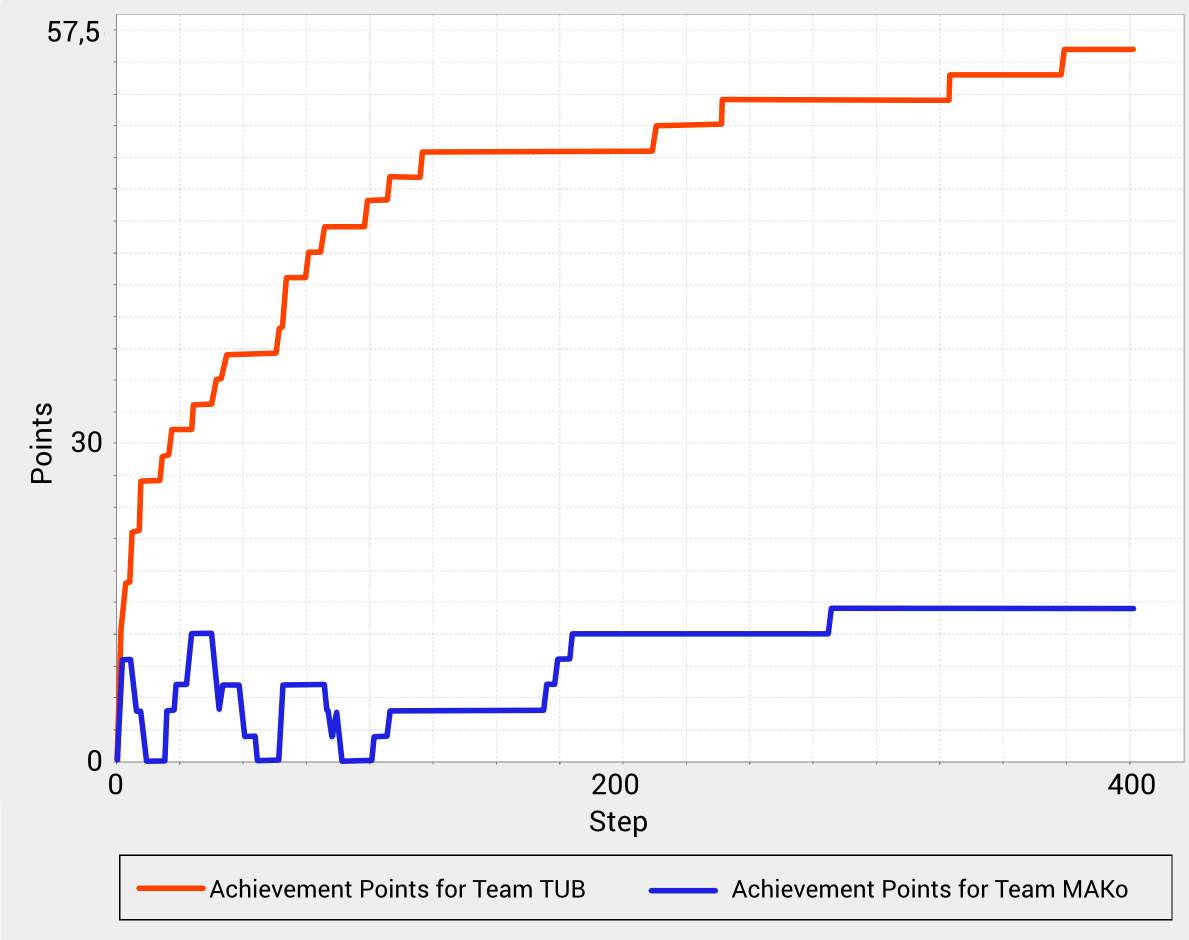
\includegraphics[width=\textwidth]{images/AchievementPoints.png}
	\caption{Achievement points from the second match TUB against MAKo.} % TODO I just wrote second as a filler. What match was it?
	\label{dis:achievement_points}
\end{figure}
On first sight, one could assume that this strategy was a drawback because achievement points earned at some point count into every future step score.
But compared to the number of points awarded for zones, the achievement points are only a minor fraction of the step score.
As it can be seen in \autoref{dis:ZonesScoresAndAchievementPoints} the spending of achievement points did not interfere dramatically with the overall score.
It was worth spending the achievement points for the purpose of attacking and disturbing the other team.
This was because the amount of potential zone points they would have earned without being attacked, would probably have been much higher than the amount of achievement points team MAKo spent for upgrades.
\begin{figure}[h]
	\centering
	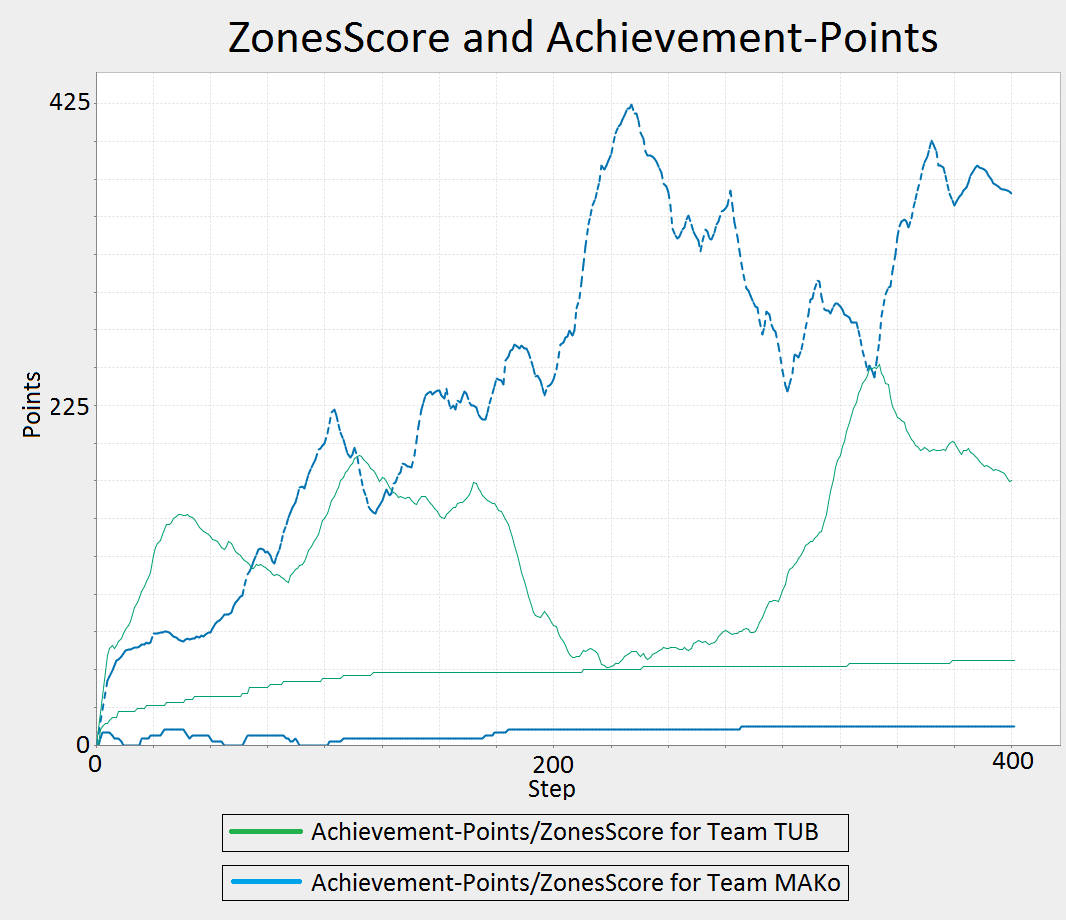
\includegraphics[width=\textwidth]{images/ZonesScoresAndAchievementPoints.png}
	\caption{Combined achievement and zone scores from the second match TUB against MAKo.} % TODO I just wrote second as a filler. What match was it?
	\label{dis:ZonesScoresAndAchievementPoints}
\end{figure}
At the end of the tournament team MAKo scored second with a total of 18 points.
The winner of 2014 was, for the third time in a row, the team from the Federal University of Santa Catarina (UFSC).
The final results are shown in~\autoref{tab:mapc2014results}.
\begin{table}[ht]
  \centering
  \label{tab:mapc2014results}
  \begin{tabularx}{\textwidth}{| l | X | p{2cm} | X | p{2cm} | l |}
    \hline
    \textbf{Pos.} & \textbf{Team name} & \textbf{Country} & \textbf{Score}       & \textbf{Difference} & \textbf{Points} \\ \hline
    1             & SMADAS-UFSC        & Brazil           & 1180662 : 654624     & \ 526038            & 33              \\
    2             & MAKo               & Germany          & \ \ 617086 : 776868  & -15782              & 18              \\
    3             & TUB                & Germany          & \ \ 904874 : 872399  & \ 32475             & 15              \\
    4             & TheWonderbolts     & Denmark          & \ \ 711001 : 1014669 & -303668             & 15              \\
    5             & GOAL-DTU           & Denmark          & \ \ 653178 : 748241  & -95063              & 9               \\ \hline
    % \phantom will generate a newline for some reason so I had to replace it with \
  \end{tabularx}
  \caption{The results of the 2014 MAPC. Each team played three matches against every other team, and winning a match awarded 3 points.}
\end{table}
Statistics of all the individual games can be found in the appendix.[reference here!!!!] % TODO I'm unsure what all you want to add here. But I'll just add this todo here so that we can grep for TODOs in the document itself :)

Our team MAKo lost every second game against all opponents.
This was due to the repairer agents not being able to repair.
We were unable to figure out why this problem arose.
But we found out that manually restarting our agents solved the problem.
Unfortunately as a result, the knowledge about the graph acquired by the agents prior to restarting was reset.
Consequently, the agents surveyed and probed redundantly.
This behaviour was especially surprising as our agents fully restarted automatically after each round and there were no such problems in all third rounds.
The restarts were all manually supervised and showed no sign of failure at any time.

Disregarding this problem, our matches can be summarised as the follows.
Our agents successfully explored the map, repaired disabled agents and attacked the opponent.
Once our designated artillery agent had stopped upgrading, it did not have to move much anymore.
Instead, it effectively attacked distant enemies and recharged mainly to attack afterwards again.
This and the other saboteur agents which were always in search for enemy agents to attack helped disturb the zone building of the other teams.
First, disabled agents were not able to build zones.
Second, disabled agents needed to be repaired which could make the repairer agents temporarily unusable for zoning depending on the strategy the enemies implemented.
If the enemy repairer agents moved towards disabled agents, they could break up a zone which they had been in earlier.

While monitoring the competition, we saw that zoning was subpar.
Due to the fact that zones were broken up periodically, zones with a high value were sometimes discarded even when there was no need to.
Furthermore, the asynchronous communication during zone finding did not work as well as hoped for.
This was partly related to our agents being attacked and disabled by enemy agents.
Agents which ought to form a zone unpredictably had to cancel their zoning availability and get repaired.
Also, we did not implement an algorithm to detect the ``end'' of the graph, say the edges of the map.
In the course of the matches, we saw that multiple maps favoured such an approach.
Being able to detect these ``ends'' would have enabled us to form greater zones with fewer agents than what our algorithm calculated.
% TODO: maybe we should add a picture explaining this. I imagine a screenshot of a graph of the last match with some highlight where to place that one special agent. I'll might create this later on.
Nevertheless, the general idea regarding small zone forming proved to be a good choice.
One big zone would have been easy to disturb.
But having multiple small high value zones was quite effective in not providing the enemy with an easy target.
% TODO: these are from the TOC:
%What place did we rank? How did the others do? Analyse our matches shortly and point out problems we faced, how we tackled them and point out what had gone well.
